\tikzstyle{init} = [pin edge={to-,thin,black}]
\tikzstyle{circ} = [circle, minimum size=1cm, text centered, draw=black, fill=blue!20]
\tikzstyle{arrow} = [thin,->,>=stealth]

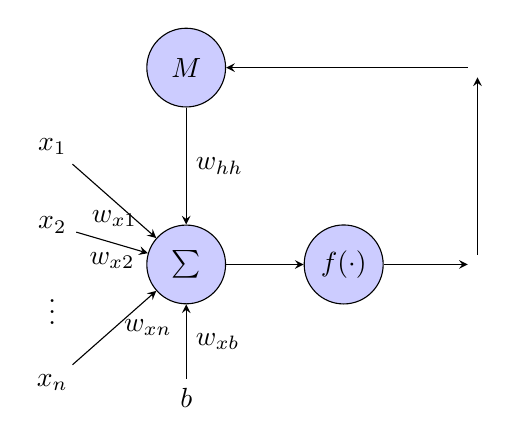
\begin{tikzpicture}
    % Perceptron
    \node (x1)    [init] {$x_1$};
    \node (x2)    [init, below of=x1] {$x_2$};
    \node (vdots) [init, below of=x2] {$\vdots$};
    \node (xn)    [init, below of=vdots] {$x_n$};
    
    \node (sum)    [circ, right of=x2, xshift=0.7cm, yshift=-5mm] {$\sum$};
    \node (b)      [init, below of=sum, yshift=-0.7cm] {$b$};
    \node (obj)    [circ, right of=sum, xshift=1cm] {$f(\cdot)$};
    \node (output) [init, right of=obj, xshift=0.7cm] {};
    \node (empty1) [init, above of=output, yshift=1.5cm] {};
    \node (lstm)   [circ, above of=sum, yshift=1.5cm] {$M$};
    
    \draw [arrow] (x1) --node[anchor=north] {$w_{x1}$} (sum);
    \draw [arrow] (x2) --node[anchor=north] {$w_{x2}$} (sum);
    \draw [arrow] (xn) --node[anchor=west] {$w_{xn}$} (sum);
    \draw [arrow] (b) --node[anchor=west] {$w_{xb}$} (sum);
    \draw [arrow] (sum) -- (obj);
    \draw [arrow] (obj) -- (output);
    \draw [arrow] (output) -- (empty1);
    \draw [arrow] (empty1) -- (lstm);
    \draw [arrow] (lstm) --node[anchor=west] {$w_{hh}$} (sum);
\end{tikzpicture}